%!TEX encoding = UTF-8 Unicode
\documentclass{article}
\usepackage{jim,amsmath}
\usepackage[T1]{fontenc}
\usepackage[francais]{babel}
\usepackage{cite}
\usepackage{fancyvrb}
\usepackage{verbatim}
\usepackage{relsize}
\usepackage{graphicx}
\usepackage[utf8]{inputenc}
\usepackage[francais]{babel}
\usepackage{hyperref}
\usepackage{hypcap}

\usepackage{graphicx}
\usepackage{graphviz}

% Title.
% ------
%\def\papertitle{A RELATIONAL MODEL FOR COMPUTER-BASED MUSIC ENGRAVING}
%\def\firstauthor{Mike Solomon}
%\def\secondauthor{Dominique Fober}

\title{Un modèle relationnel de la gravure musicale}

\twoauthors
  {Mike Solomon} {ensemble 101 \\ \href{mailto:mike@ensemble101.fr}{mike@ensemble101.fr}}
  {Dominique Fober} {Grame \\ \href{mailto:fober@grame.fr}{fober@grame.fr}}

\begin{document}
%
\capstartfalse
\maketitle
\capstarttrue
%
\begin{abstract}
Cet article a pour objet d'élaborer un modèle relationnel de la gravure
musicale. Les bases de données relationnelles, de plus en plus répandues
comme solution de stockage de données,
permettent de résoudre des problèmes d'indépendance et
de incohérence des données qui entravent la migration vers le web des
logiciels de gravure musicale. Cette conception relationnelle de la partition
musicale permet également de faire des projections arbitraires des partitions
dans plusieurs contextes numériques. Après avoir survolé l'état de l'art de
la gravure musicale assistée par ordinateur, l'article propose un modèle relationnel de la
gravure avant de conclure avec une discussion sur le lien entre le modèle
relationnel et d'autres systèmes d'encodage musical.
\end{abstract}
\section{Introduction}
Depuis la création du logiciel SCORE pendant les années
1970~\cite{smith1972score}, la gravure musicale assistée par ordinateur fait
partie des problématiques les plus étudiées en informatique musicale.
Le domaine regroupe plusieurs axes de recherche dont les systèmes de
représentation musicale~\cite{good2003using}\-\cite{hoos1998guido}\-\cite{good2001musicxml},
la modélisation de la gravure classique par le biais
d'algorithmes~\cite{hegazy1988optimal}\-\cite{blostein1991justification},
les interfaces utilisateurs qui permettent de travailler facilement avec
la notation et la lecture musicale à partir des écrans d'ordinateur~\cite{fitzpatrick1998networked}\-\cite{qian2002portable}\-\cite{egyud1998hand}.
\begin{figure}[h]
\begin{Verbatim}[frame=single,fontsize=\relsize{-1}]
\relative c'' {
  a16-.\fp [ b-. c ( d ] e8.\espressivo\< )
  [ fis,16->\f ] c'4.\fermata r8 \bar "|."
}
\end{Verbatim}
\begin{center}
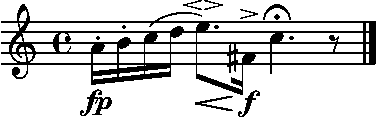
\includegraphics{example_preview.pdf}
\end{center}
\caption{Syntaxe d'entrée de GNU LilyPond et la partition à laquelle le
texte conduit une fois compilé.}
\end{figure}

Avec l'apparition récente des plate-formes web d'édition musicale~\cite{renz1998web}\-\cite{solomon2014deploiement},
la gravure musicale assistée par ordinateur doit faire face à de nouveaux
défis techniques dont l'édition à plusieurs~\cite{jorda2001system}\-\cite{bainbridge1999towards}\cite{viro2011peachnote}
et l'encapsulation de la logique des logiciels d'édition dans des widgets interactifs
embarquables dans de plus grands contextes numériques~\cite{agon2002programmation}\-\cite{laurson2002pwgl}\-\cite{guedy2013etudier}, notamment dans un navigateur web.
Cette tendance va à l'encontre des programmes autonomes de gravure musicale
qui dominent le marché actuel. Un manque d'inertie dans la modernisation de
ces logiciels provient largement de l'absence d'un modèle de représentation musicale
qui permet de faire des projections arbitraires d'une partition (une
sélection de mesures, un groupe de portées, les notes les plus aigües de chaque
voix, etc.) dans
plusieurs contextes d'affichage. Cet article propose une solution tripartite
à ce problème :
\begin{itemize}
\item Un modèle relationnel de représentation musicale qui s'adapte facilement à de
différents environnements numériques (Section~\ref{sec:communication}).
\item Un protocole de communication qui permet aux données musicales dans
ce système d'être transmises facilement entre plusieurs clients
(Section~\ref{sec:definition}).
\item Un ensemble de recommandations pour la création d'une librairie,
écrite en SQL, qui permet d'effectuer la gravure selon ce modèle (Section~\ref{sec:library}).
\end{itemize}
Après avoir survolé l'état de l'art de la gravure musicale assistée par ordinateur,
l'article élabore les éléments clés d'un modèle relationnel de la gravure
musicale. Il conclut avec une discussion sur la pertinence de cette méthode
dans le paysage global des applications musicales sur le web et des
systèmes d'encodage de la musique.

\section{L'état de l'art}
L'état de l'art de la gravure musicale assistée par ordinateur se décline selon trois
axes de développement principaux: les modèles de représentation musicale,
les algorithmes de mise en page et les méthodes de visualisation des
partitions.
\subsection{Modèles de représentation musicale}
Il existe actuellement trois modèles communément utilisés de représentation musicale 
 -- les langages de balisage exploitables dans plusieurs applications, les syntaxes
d'entrée textuelles pour des éditeurs
et les représentations internes de la musique associées
principalement aux éditeurs graphiques. Les langages génériques, dont abc
\cite{duggan2008system}, MusicXML \cite{good2001musicxml}
et Music Encoding Initiative (MEI) \cite{roland2002music} proposent
des conteneurs hiérarchiques (instrument, portée, accord, etc.) pour la
modélisation de la musique. Les syntaxes liées à des éditeurs comme
ceux qui embarquent libGUIDOEngine \cite{hoos1998guido},
MusicTeX \cite{taupin1993musictex} et
GNU LilyPond \cite{nienhuys2002gnu} se basent sur un langage se rapprochant
de celui de \TeX{} alors que des projets comme Common Music
Notation (CMN) \cite{schottstaedt1997common} et Abjad
\cite{trevino2014automated} se servent largement des langages d'extension
LISP et Python pour définir un format d'entrée musicale.
Plusieurs systèmes de représentation existent à l'intérieur de ces logiciels
afin de regrouper, ordonner et traiter les objets musicaux avant d'effectuer la mise en page. La
plupart de logiciels utilisent un système orienté objet (MuseScore,
GUIDO) qui attribue des propriétés à des objets graphiques (altérations,
clefs, hampes etc.) tandis qu'une minorité utilise la programmation fonctionnelle (CMN, LilyPond)
pour représenter la musique comme un flot d'évènements à traiter par une série
de fonctions \cite{sandberg2006separating}.
\subsection{Algorithmes de mise en page}\label{sec:layout_algorithms}
Les algorithmes de mise en page musicale peuvent être classés dans deux
groupes principaux : les algorithmes coûteux et affinés pour les langages musicaux
compilés et les algorithmes plus rapides et moins précis pour la mise en
page en temps réel. La plupart de langages compilés s'efforcent de suivre
les recommandations d'espacement musical soulignés par
Read \cite{Read64}, Ross \cite{Ross70} Gould \cite{Gould11} et d'autres
graveurs reconnus.
Les travaux de Gourlay \cite{Gourlay87}, Haken et Blostein
\cite{Haken91} et Renz \cite{Renz02} traduisent ces textes en algorithmes
d'espacement qui s'inspirent largement de l'algorithme \emph{boîte et colle}
proposé par Kunth dans \TeX \cite{Kunth81}. Les logiciels proposant une mise
en page en temps réel, comme MuseScore et NoteFlight, utilisent une
variation de l'algorithme glouton de sauts de ligne utilisé par la plupart
d'éditeurs de texte graphique et les engins de rendu de texte dans les
navigateurs web.
\subsection{Visualisation de la partition}
Dans la plupart d'éditeurs survolés ci-dessus (MuseScore, LilyPond, GUIDO,
CMN), la visualisation de la partition sur un écran d'ordinateur est
étroitement lié à l'impression éventuelle de la partition sur un support
papier. Plusieurs technologies existent également pour la visualisation
des partitions musicales sur des appareils d'affichage numériques, notamment
des logiciels qui font défiler une partition pendant un concert de musique~\cite{fitzpatrick1998networked}\-\cite{qian2002portable}\-\cite{egyud1998hand}.
Il existe également des éditeurs qui calque l'espacement horizontal d'une
partition sur la forme d'onde d'un enregistrement (Apple Logic, Finale, Antescofo).
Des widgets interactifs de gravure musicale existent également dans des langages de
programmation visuelle utilisées pour la génération du son et de la vidéo (Pd,
Max/MSP) et pour la composition musicale (OpenMusic, PWGL).
Les fenêtres de gravure ouvrables dans ces environnements de programmation
visuelle s'adaptent à la logique
des langages de programmation, s'intégrant souvent dans un flot de données pour
pouvoir visualiser un processus sonore ou le résultat d'un algorithme
génératif. Ils doivent faire face à de lourdes contraintes de taille et de
vitesse~\cite{kelly2011gemnotes}
pour pouvoir calculer et afficher rapidement des partitions. 
Dans l'Expressive Notation Package (ENP)
\cite{kuuskankare2006expressive}, cette idée est élaborée dans un espace
musical multidimensionnel où chaque visualisation affichée sur l'écran correspond à
une vicissitude différente de la partition (esquisse de compositeur, partition d'interprète, etc.).

\section{Un modèle relationnel de la gravure musicale}
Bien que l'état de l'art propose un riche ensemble de logiciels de gravure,
aucun logiciel n'est adapté ni à l'affichage des partitions sur Internet en
temps réel, ni à l'édition à plusieurs. Pour combler cette
lacune, le présent article propose un système de gravure musicale assistée par
ordinateur basé sur le
\emph{modèle relationnel}.
Dans ce modèle, les données liées aux objets graphiques de la partition sont
stockées dans une base de données relationnelle et modifiées par le biais
d'opérations d'algèbre relationnelle. Des applications externes récupèrent
les résultats de ces calculs afin d'effectuer la mise en page des objets
musicaux.
Cette section avancera l'hypothèse que les éléments graphiques d'une partition
musicale peuvent être encodés, manipulés et partagés de façon expressive et
succincte dans le cadre ce modèle.\par
\subsection{Définition du modèle relationnel}\label{sec:definition}
Le modèle relationnel \cite{codd1970relational}, élaboré par IBM pendant les
années 1960, répondait à l'époque à un besoin de séparer les
représentations internes des données et les opérations sur ces données comme
insérer, supprimer, modifier et interroger. Les deux buts principaux du
modèle relationnel sont la gestion de l'\og{} \emph{indépendance des
données}--l'indépendance des logiciels visuels et des utilités de ligne de commande
par rapport à la représentation interne des données--et certaines formes
d'\emph{incohérence des données} qui nuisent au fonctionnement de plusieurs
systèmes de calcul, y compris les systèmes non inferentiaux\fg{}
\cite[p.377]{codd1970relational}. Si l'indépendance des données permet à
de différents clients de travailler de façon asynchronée
à partir d'un noyau central de données,
l'incohérence des données arrive quand les mêmes données sont exploitées de
manière différente selon le client.\par
Le modèle relationnel résout ces deux problèmes en joignant de façon
dynamique un ensemble de données
à un ensemble de relations. Le mot \og{}relation\fg{} est utilisé dans le sens
mathématique classique du terme: il s'agit d'un ensemble de \emph{n}-uplets où, pour
chaque indice \emph{i} d'un \emph{n}-uplet, la valeur à cette indice existe dans
un ensemble $S_{i}$. Plus intuitivement, un \emph{n}-uplet est un rang dans
une base données. Les rangs, superposés, créent des colonnes qui
correspondent aux ensembles $S_{i}$. Bien que l'analogie de colonnes et de
rangs soit utile, le modèle relationnel ne préconise aucun système de
stockage interne des données. Grâce à cette définition abstraite de
l'organisation des données, les clients qui interrogent le système
n'ont pas besoin de savoir le schéma de représentation à
l'intérieure de la base de données.  Autrement dit, les données et les
applications sont \emph{indépendantes}. Quant à l'\emph{incohérence} des
données, s'il existe une relation 
$R_{1}$ entre Employée et Prénom et une deuxième relation $R_{2}$
entre Employée et Nom de famille, une application n'est pas obligée de
définir le prénom et le nom de famille afin de représenter la personne dans
le système. Le sens des relations n'est pas imposé par le modèle
relationnel mais plutôt par les applications qui interrogent la base de données. Ça
permet aux logiciels travaillant avec la base de données de ne stocker que les
données dont ils ont besoin et d'utiliser ces données pour des fins
différentes.
\subsection{La partition musicale comme ensemble de relations}
Tous les textes phares de la gravure musicale définissent un ensemble de relations
géométriques plus ou moins strictes entre des symboles musicaux. Par
exemple, dans \emph{Behind Bars} de Gould \cite{Gould11}, l'on trouve
plusieurs phrases comme celle-ci:
\begin{quote}
Pour éviter les collisions entre les liaisons et les articulations ou les
liaisons de phrasé, il faut que les bouts de la liaison soient alignés aux
bords des têtes de note. Sinon, il faut que la liaison commence juste
après la première tête de note et qu'elle se termine juste avant la deuxième.
\cite[p.62]{Gould11}\\
\begin{center}
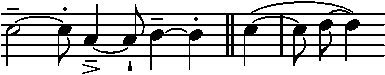
\includegraphics{gould_preview.pdf}
\end{center}
\end{quote}
A l'intérieur de ce constat se trouve de nombreuses relations -- tête de
note et articulation, tête de note et liaison de phrasé, tête de note et
liaison, liaison et articulation etc. Un modèle relationnel permet d'englober
plusieurs règles du même genre sans hiérarchiser les rapports entre les
objets. Par exemple, on ne précise pas qu'une articulation fait partie d'une note ou vice
versa -- il faut tout simplement établir un ensemble de relations et la gravure
musicale est le résultat graphique qui découle de ces contraintes. Il ne
faut pas non plus établir un ensemble d'objets de notation musicale
\og{}essentiels\fg{} que tous les clients doivent savoir trier.
Un logiciel de gravure qui ne propose pas de liaisons de phrasé, par
exemple, peut omettre
les relations concernant cet élément graphique sans compromettre les autres
relations.\par
\subsection{Communication dans le modèle relationnel}\label{sec:communication}
Le modèle relationnel de la gravure musicale assistée par ordinateur
permet d'effectuer des opérations sur les données par le biais de l'algèbre
relationnelle \cite{codd1970relational}. Cette algèbre comprenait au départ
cinq opérations (permutation, projection, jointure,
composition et restriction) auxquelles s'ajoutent trois opérations
supplémentaires (jointure externe, projection étendue, et fermeture
transitive) dans Structured Query Language (SQL) \cite{date2011sql} --
un format d'échange mondialement répandu pour manipuler et interroger des bases de
données relationnelles.\par
L'un des avantages majeurs de l'algèbre relationnelle est sa capacité
d'exprimer des effets d'interférence qui sont difficiles à
préciser dans une organisation hiérarchique des connaissances. Par exemple,
dans la gravure traditionnelle, une liaison de phrasé peut influer sur
l'espacement vertical d'une articulation et une indication de nuance.
(Figure~\ref{figure:slur_d_a}).
\begin{figure}
\begin{center}
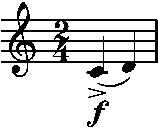
\includegraphics{slur_dynamic_articulation}
\end{center}
\caption{Une liaison de phrasé qui arrive au même moment qu'une indication
de nuance et un symbole d'articulation.}
\label{figure:slur_d_a}
\end{figure}
Or, plusieurs textes sur la gravure musicale (\cite{Read64}\-\cite{Ross70}\-\cite{Gould11}) traitent
les courbes et les symboles d'expressivité dans de différents chapitres,
n'exposant que superficiellement les
multiples relations qui peuvent survenir entre ces éléments graphiques. En
général, les supports qui obligent à hiérarchiser les connaissances, comme
les livres et les pages web, ne sont pas bien adaptés aux domaines qui
doivent prendre en compte beaucoup d'effets d'interférence. Avec l'algèbre
relationnelle (Figure~\ref{figure:sql}), les relations peuvent encadrer des effets
transversaux entre plusieurs éléments,
permettant de
modéliser facilement des effets d'interférence dans l'espacement des objets
graphiques que représentent les données.
\begin{figure}
\begin{Verbatim}[frame=single,fontsize=\relsize{-1}]
SELECT y_position.val
FROM y_position
  JOIN x_position
    ON y_position.id = x_position.id
  JOIN name
    ON y_position.id = name.id
WHERE name = 'articulation'
  OR name = 'dynamic'
  OR name = 'slur';
\end{Verbatim}
\caption{Pseudo-code en SQL qui récupère les coordonnées Y des liaisons,
nuances et articulations simultanées.}
\label{figure:sql}
\end{figure}
\section{purcell: Une librairie relationnelle
de gravure musicale assistée par ordinateur}\label{sec:library}
Le projet \Verb[fontsize=\relsize{-0.5}]=purcell= propose une mise en œuvre
du modèle relationnel de la gravure assistée par ordinateur.
\Verb[fontsize=\relsize{-0.5}]=purcell= est basé sur un ensemble de tables liées par le biais de
relations écrites en SQL auxquelles on peut accéder en passant par des
websockets, le HTTP et l'OSC.
Les relations SQL sont des \emph{relations déclencheuses} qui induisent
d'autres relations si certaines conditions sont réunies.
\begin{figure}
\begin{center}
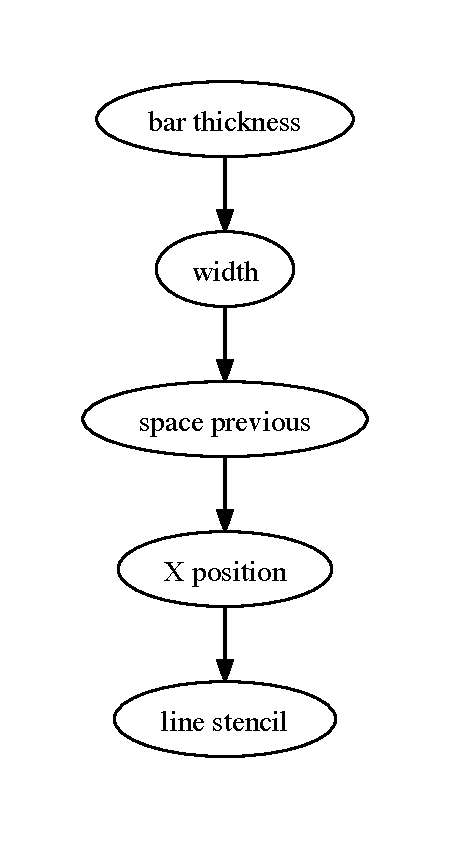
\includegraphics[width=4cm]{flowchart}
\end{center}
\caption{Le cheminement du déclenchement des tables dans une base de données
relationnelle qui modélise la gravure musicale. La chaîne commence
avec l'épaisseur d'une
barre de mesure (bar thickness) et procède jusqu'à sa représentation graphique
(line stencil) en passant par
la largeur totale de l'objet (width), l'espace entre cet objet et celui à gauche
sur la portée (space previous) et le positionnement sur l'abscisse (X
position).}
\label{figure:flowchart}
\end{figure}
\begin{figure}
\begin{Verbatim}[frame=single,fontsize=\relsize{-1}]
CREATE TRIGGER bar_thickness_to_width
  AFTER INSERT ON bar_thickness
    WHEN (EXISTS (SELECT bar_thickness.id
                    FROM bar_thickness))
      BEGIN
          DELETE FROM width
                 WHERE width.id = new.id;
          INSERT INTO width (id, val)
             WITH bar_lines_to_widths AS
               (SELECT bar_thickness.id AS id,
                       bar_thickness.val AS val
                 FROM bar_thickness
                 WHERE bar_thickness.id = new.id)
             SELECT bar_lines_to_widths.id,
                    bar_lines_to_widths.val
               FROM bar_lines_to_widths;   
      END;
\end{Verbatim}
\caption{Le code SQLite qui correspond au déclenchement d'un changement
de largeur d'une barre (width) issue d'un changement d'épaisseur de barre,
soit la première flèche de la Figure~\ref{figure:flowchart}. Dans ce
déclenchement, le processus
est trivial puisque l'épaisseur du trait est copié à la table de largeur.}
\label{figure:barline}
\end{figure}
Par exemple, la
modification de la table \og{}hauteur\fg{} déclenche une modification de la
position verticale d'un objet sur une portée. Les déclenchements successifs
cheminent au remplissage des tables \og{}finales\fg{} qui indiquent les informations graphiques
associées aux
objets (points d'ancrage, coordonnées des sommets etc.). Les
contenus de ces tables sont envoyés au client qui effectue la
dernière étape de dessin des objets à partir des données fournies par la
base de données SQL. D'éventuelles modifications à la partition sont effectuées uniquement par le
biais d'opérations d'algèbre relationnelle (Figure~\ref{figure:puresql}).\par
Le projet \Verb[fontsize=\relsize{-0.5}]=purcell= a pour but de proposer des
widgets interactifs intégrables dans les logiciels musicaux indiqués dans la
Table~\ref{table:languages} d'ici 2017.
\begin{table}[h!]
\centering
\begin{tabular}{l|l}
Project & Languages \\\hline
OpenMusic & C++\\
PWGL & C++\\
InScore & C++, GUIDO\\
Faust WebAudio & C++, JavaScript, HTML, SVG\\
MediaWiki & JavaScript, HTML, SVG\\
\end{tabular}
\caption{Plate-formes de composition et édition musicales dans lesquelles la
librairie sera embarqué.}
\label{table:languages}
\end{table}
Pour visualiser une preuve de concept de \Verb[fontsize=\relsize{-0.5}]=purcell=
écrite en HTML5, veuillez consulter:
\begin{center}
\fbox{\url{http://www.mikesolomon.org/purcell}}
\end{center}
\section{Conclusion: la toile et l'encodage musical}
Dans la mesure où \Verb[fontsize=\relsize{-0.5}]=purcell= peut fonctionner
en mode serveur-client, il est bien adapté aux
exigences des plate-formes d'édition musicale sur Internet. Il est conçu
notamment pour l'utilisation décentralisée à plusieurs comme les éditeurs
textuels de Google Doc et de Framapad. Grâce à la librairie
\Verb[fontsize=\relsize{-0.5}]=sql.js=\footnote{\url{http://github.com/kripken/sql.js/}},
\Verb[fontsize=\relsize{-0.5}]=purcell= peut être utilisé comme application
client dans un navigateur sans communiquer avec un serveur central.\par
Le modèle relationnel de la gravure musicale fait partie de l'écosystème
général des langages d'encodage des partitions musicales. Grâce à ses aspects non
hiérarchiques et déstructurés, il peut schématiser les données
provenant d'autres systèmes d'encodage musical sans dénaturer
l'information. Les divergences entre plusieurs systèmes de
représentation musicale (MusicXML, MEI etc.) sont une forme
d'\emph{incohérence de données} que le modèle relationnel peut encapsuler, permettant
de gérer plusieurs systèmes d'encodage simultanément dans la même base
de données. Le modèle relationnel peut fournir donc une passerelle entre
plusieurs formats d'encodage musical, voire générer des données de
méta-encodage qui révèlent les tendances d'encodage de plusieurs clients
travaillant avec de différents formats d'entrée de données.
\begin{figure}
\begin{center}
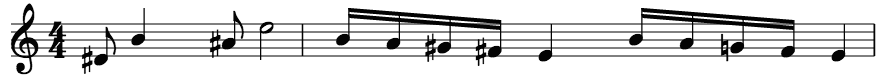
\includegraphics[width=8cm]{../JIM_2015/purcell1.png}
\end{center}
\Verb[fontsize=\relsize{-0.5}]&UPDATE accidental SET val = -1 WHERE val = 1;&
\begin{center}
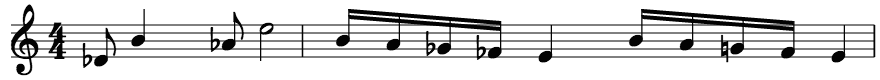
\includegraphics[width=8cm]{../JIM_2015/purcell2.png}
\end{center}
\caption{Une partition purcell générée en SVG suivie par une requête SQL et
la modification qui en découle.}
\label{figure:puresql}
\end{figure}
\bibliographystyle{plain}
\bibliography{researchProposal,moreresearch}

\end{document}
